\chapter{Resultaten}
De algoritmes worden getest in een on-line situatie gegenereerd door de simulatie. Er is enkel ruis toegevoegd op het koppel geleverd door de fietser. De modellen beginnen van nul (niet vooraf getraind). Gedurende een startperiode leren de algoritmes bij en zal de cadans bepaald worden door het fietsersmodel. De algoritmes nemen deze instelling over na de startperiode. Na elke voorspelling wordt de \gls{mse} berekend tussen de voorspelling en het fietsersmodel. Elke 30 iteraties (aan 10Hz) wordt er afgewogen of de algoritmes te ver afwijken van het fietsersmodel. Wanneer de absolute fout de grens van vijf rpm overschrijdt, zal er geleerd worden. De data gebruikt om bij te leren bestaat uit de toestand van de fiets van de afgelopen 100 iteraties (10s). Dit is arbitrair gekozen. In sommige situaties zal de vorige tien seconde aan data relevant zijn (bijvoorbeeld op een kleine helling), maar soms ook niet (bij een grote helling). Deze data wordt verwerkt tot een set van training instanties met elk een sequentie lengte n, zijnde data van iteratie 0-n,1-(n+1),..., (99-n)-99 vormt de trainingsdata gegenereerd door één keer op de knop te duwen. Deze set wordt toegevoegd aan de trainingsset die gebruikt wordt door de algoritmes. De doelvariabele die bij elke observatie hoort, is de FCC gegenereerd door het fietsersmodel. De doelvariabele zou ook incrementeel aangepast kunnen worden (+ of - k bij update), maar dit valt buiten het doel van deze thesis. Met deze evaluatiemethode wordt er nagegaan hoe snel en hoe vaak het algoritme bijleert. Alle algoritmes worden geëvalueerd in exact dezelfde omstandigheden.

\[MSE = \frac{1}{n} \sum_{i=1}^{n} (Y_i-\hat{Y}_i)^2\]

\section{Sequentie preprocessing}
De lengte van de sequenties heeft een invloed op de resultaten. Zoals te zien op figuur \ref{fig:seqlen error} heeft een te kleine sequentie negatieve invloeden op de resultaten van PA. Hoe groter de lengte van de sequentie, hoe accurater de voorspellingen worden. De tijd die het algoritme nodig heeft om de testen te voltooien stijgt ook naargelang de grootte van de sequenties. De error en uitvoeringstijd bij DT en RF ondervinden een kleine impact bij het variëren van de lengte van de sequenties. 
\\\\
Om goede resultaten te krijgen, zetten we de lengte van de sequenties boven de 20. Wat juist de beste optie is, is moeilijk te zeggen. Een kleine sequentie omvat maar enkele omwentelingen van de pedalen. Als er hier een grote inconsistentie voordoet kan dit slechte resultaten opleveren. Daarom zullen alle testen vanaf dit punt een constant lengte van 50 hebben. 
\begin{figure}[t!]
\centering
\begin{subfigure}{.49\textwidth}
  \centering
  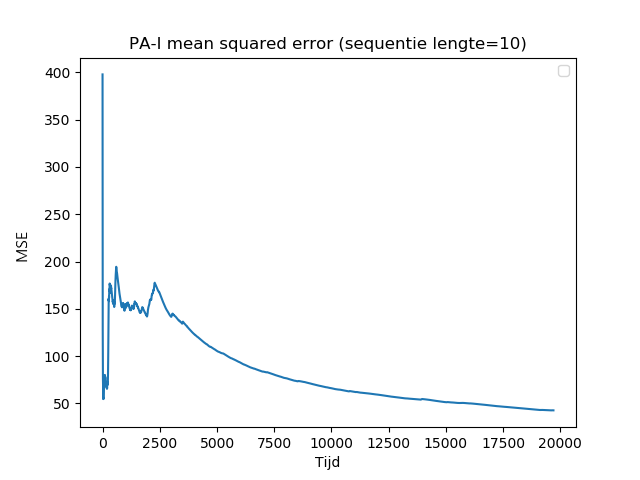
\includegraphics[width=\linewidth]{images/evaluatie/seqlen10.png}
\end{subfigure}
\begin{subfigure}{.49\textwidth}
  \centering
  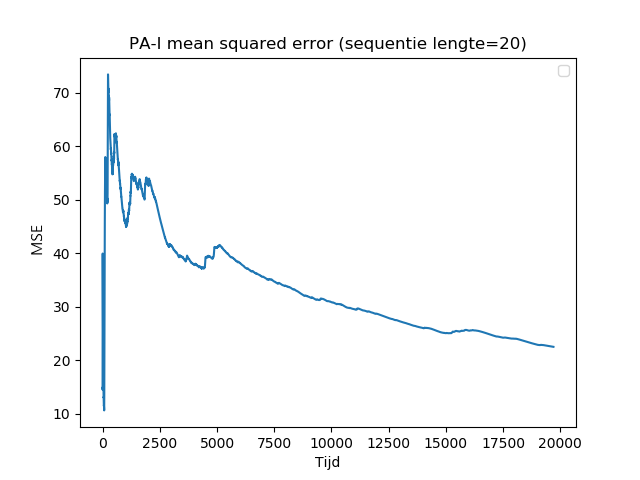
\includegraphics[width=\linewidth]{images/evaluatie/seqlen20.png}
\end{subfigure}
\begin{subfigure}{.49\textwidth}
  \centering
  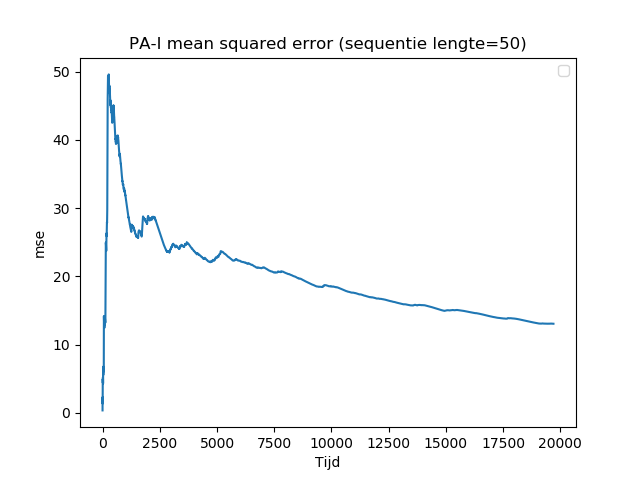
\includegraphics[width=\linewidth]{images/evaluatie/seqlen50.png} 
\end{subfigure}
\begin{subfigure}{.49\textwidth}
  \centering
  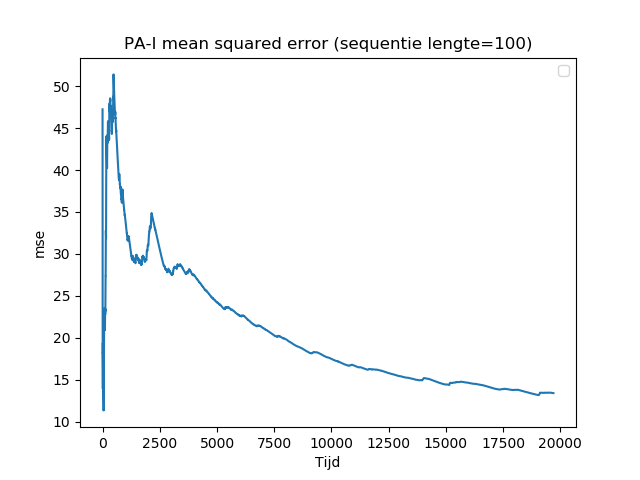
\includegraphics[width=\linewidth]{images/evaluatie/seqlen100.png}   
\end{subfigure}
\caption{De invloed van sequentielengte op de error}
\label{fig:seqlen error}
\end{figure}
\section{Algoritmes}
\subsection{Passive Aggressive Algorithm}
Er zijn enkele hyperparameters die ingesteld kunnen worden. \texttt{Max\textunderscore iter} is het maximum aantal iteraties dat het algoritme probeert bij te leren gedurent één training. \texttt{Tol} is een parameter die bepaalt of het algoritme vroegtijdig stopt. Dit gebeurt wanneer de fout na een leercyclus met minder dan \texttt{tol} verbetert. In de testomgeving, met $max\_ iter=25$ en $tol=0.1$, wordt deze vroegtijdige stop altijd behaald. Met andere woorden, na 25 iteraties heeft het algoritme de nieuwe data geleerd.
\\\\
Een laatste interessante parameter is C: de agressiviteit parameter. Hoe hoger deze is, hoe agressiever het algoritme de gewichten bijwerkt. De onderstaande figuur toont hoe de C-parameter de MSE beïnvloed van zowel PA-I als PA-II. C is de enige parameter die aangepast wordt.
\\\\
Bijna alle testen convergeren naar een MSE tussen tien en vijftien, met een gemiddelde tussen dertien en veertien. Er is geen duidelijk verschil te zien tussen PA-I en PA-II. In de paper van Crammer et al. \cite{pa algorithm} worden beide versies vergeleken op basis van instance noise en label noise. In beide gevallen scoren PA-I en PA-II aanzienlijk beter dan het standaardalgoritme. In dit experiment scoren PA-I en PA-II gelijkaardig.
\\\\
Figuur \ref{fig:gemiddeld aantal keer trainen pa} toont de invloed van C op het gemiddeld aantal keer trainen. Deze data is genomen over tien sessies, van elk 20000 iteraties. Het verschil tussen de verschillende settings is klein. De “stappen” die genomen worden tijdens het trainen zullen dus vaak klein genoeg zijn zodat C=1 agressief genoeg is. Het is dus niet nodig om hoge C-waarden (5-10) te gebruiken.
\\\\
\begin{figure}[h]
	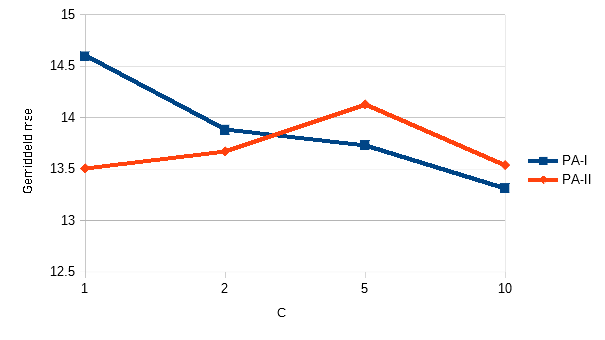
\includegraphics[width=\linewidth]{images/evaluatie/gemiddeldmsepa.png}
	\caption{De invloed van C op het gemiddeld MSE van PA}
	\label{fig:invloed C op PA}
\end{figure}
\newpage
\begin{figure}[t]
	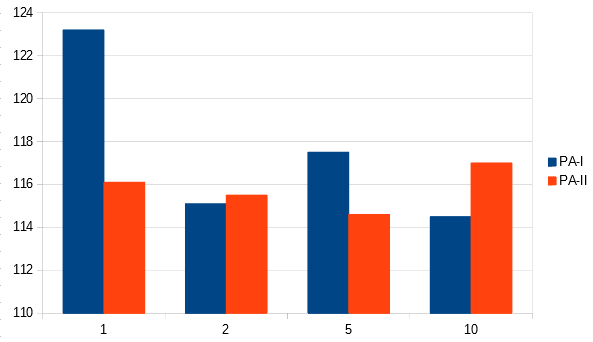
\includegraphics[width=\linewidth]{images/evaluatie/aantalkeertrainenpa.png}
	\caption{Gemiddeld aantal keer trainen PA}
	\label{fig:gemiddeld aantal keer trainen pa}
\end{figure}
\subsection{Decision Tree en Random Forest}
De belangrijkste parameter bij deze regel-gebaseerde algoritmes (\textit{rule-based learners}) is de maximum diepte. Dit is een moeilijk in te schatten parameter, vooral voor de DT. Diepere DT’s maken betere voorspellingen, maar op een bepaald punt begint de DT te overfitten. Bij RF kan ook het aantal bomen ingesteld worden. Hoe meer bomen er gebruikt worden, hoe minder invloed ruis heeft op voorspellingen en hoe beter de voorspellingen worden.
\\\\
DT’s en RF’s convergeren beide naar ongeveer dezelfde MSE. Diepere bomen leiden evident naar een lagere MSE. Algemeen zijn grotere RF’s beter, maar in deze situatie is het verschil klein.
\\\\
Voor DT daalt het gemiddeld aantal trainingen spectaculair tussen diepte drie en vier (figuur \ref{fig:invloed diepte en aantal bomen trainen}). Een DT van diepte drie zal dus geen goede oplossing zijn. RF’s daarentegen presteren wel goed met een diepte van drie. Een DT/RF dieper dan vier is niet nodig, aangezien dit geen groot voordeel oplevert en mogelijk overfit.
\\\\
De uitvoeringstijd (figuur \ref{fig:invloed diepte en aantal bomen uitvoeringstijd}) lijkt geen probleem te vormen voor grotere RF en stijgt zoals verwacht. Bij DT daarentegen, daalt de uitvoeringstijd, wat onverwacht is. Het verschil tussen de uitvoeringstijden van een DT met diepte drie en de andere is te wijten aan het aantal keer dat getraind moet worden op diepte drie. Bij diepte drie ligt dit veel hoger dan de andere dieptes.

\begin{figure}[htp!]
\centering
\begin{subfigure}{\textwidth}
  \centering
    \hspace*{-0.75cm}                                                           
  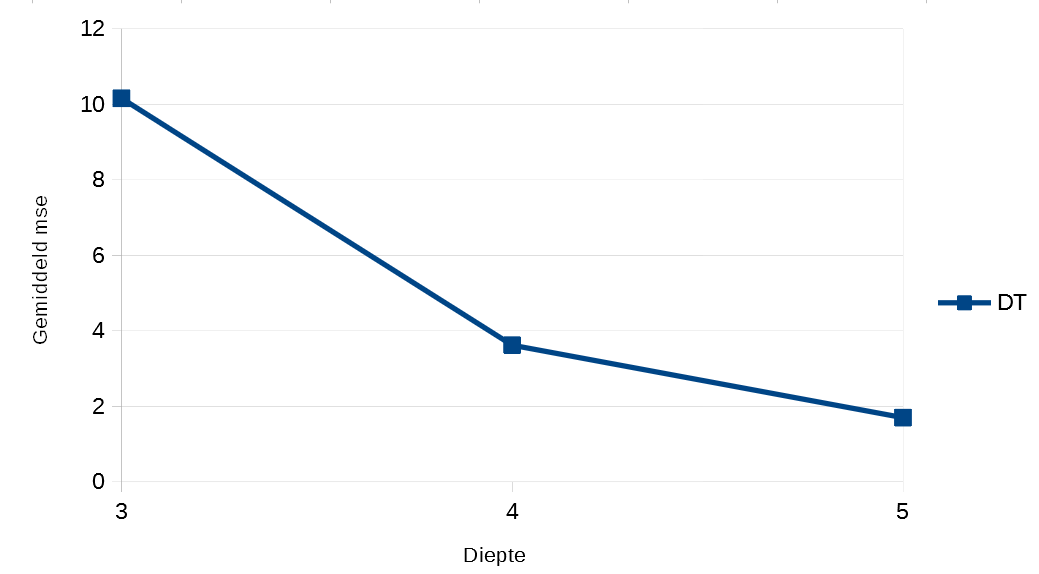
\includegraphics[width=\linewidth]{images/evaluatie/gemiddeldmsedt.png}
\end{subfigure}
\begin{subfigure}{\textwidth}
  \centering
  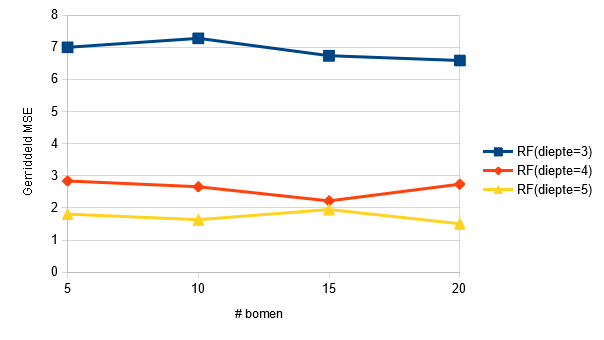
\includegraphics[width=\linewidth]{images/evaluatie/gemiddeldmserf.png}
\end{subfigure}
\caption{De invloed van diepte en aantal bomen op de gemiddelde MSE van DT en RF}
\label{fig:invloed diepte en aantal bomen mse}
\end{figure}
\begin{figure}[htp!]
\centering
\begin{subfigure}{\textwidth}
  \centering
    \hspace*{-0.75cm}                                                           
  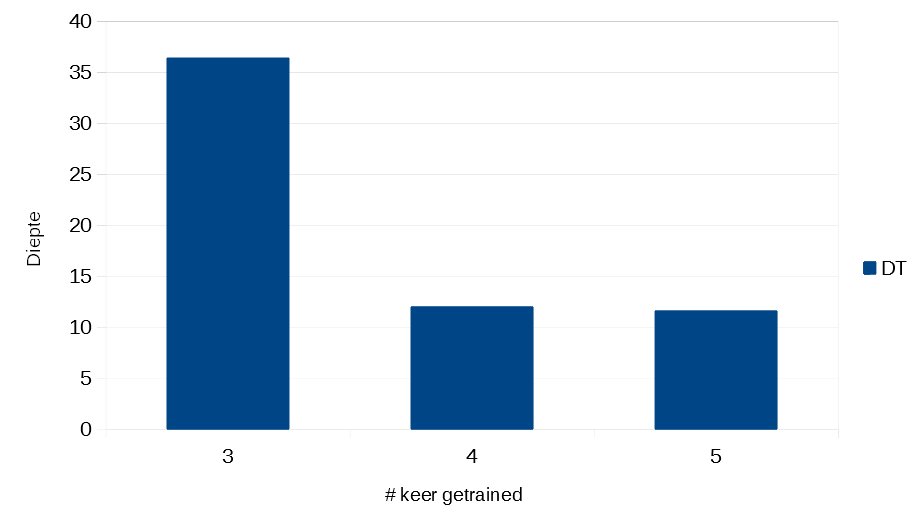
\includegraphics[width=\linewidth]{images/evaluatie/aantalkeertrainendt.png}
\end{subfigure}
\begin{subfigure}{\textwidth}
  \centering
  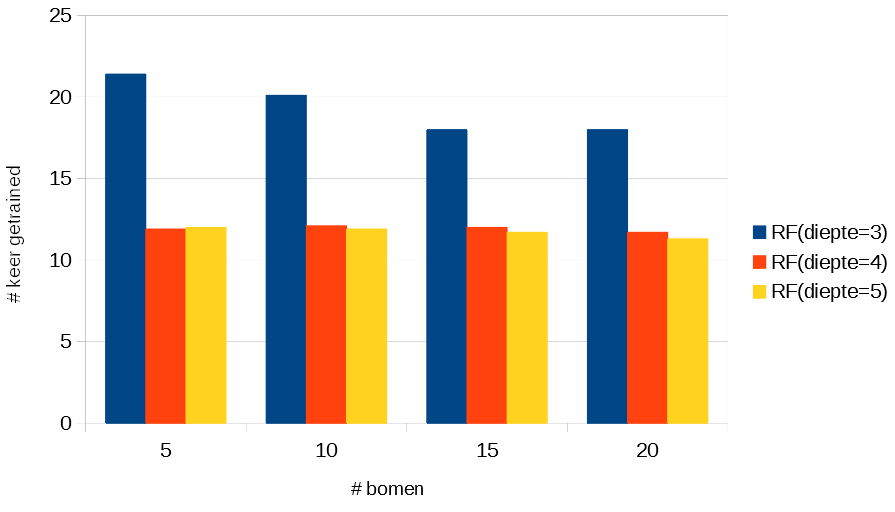
\includegraphics[width=\linewidth]{images/evaluatie/aantalkeertrainenrf.png}
\end{subfigure}
\caption{De invloed van diepte en aantal bomen op het gemiddeld aantal keer trainen van DT en RF}
\label{fig:invloed diepte en aantal bomen trainen}
\end{figure}
\begin{figure}[htp!]
\centering
\begin{subfigure}{\textwidth}
  \centering
  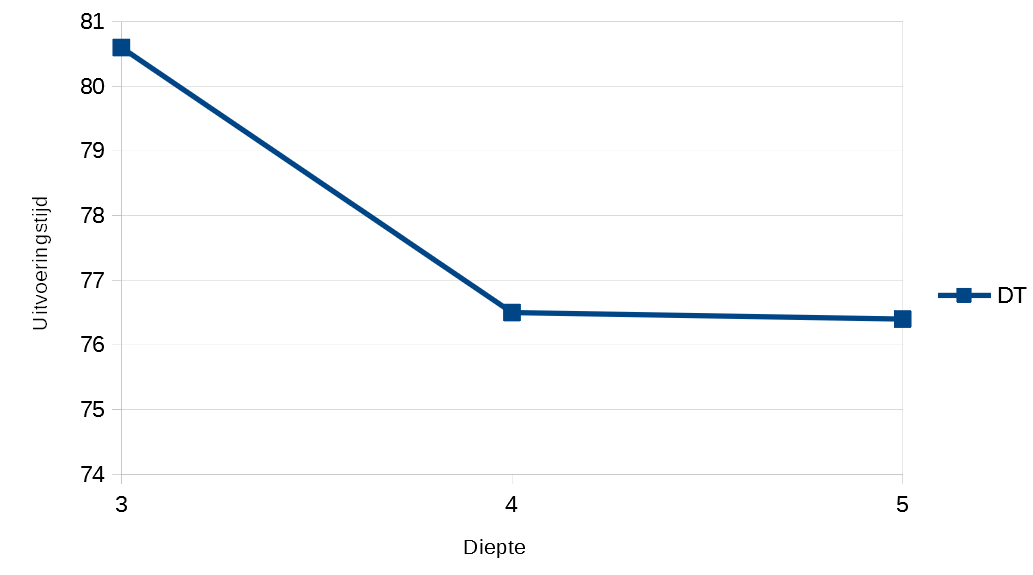
\includegraphics[width=\linewidth]{images/evaluatie/uitvoeringstijddt.png}
\end{subfigure}
\begin{subfigure}{\textwidth}
  \centering
  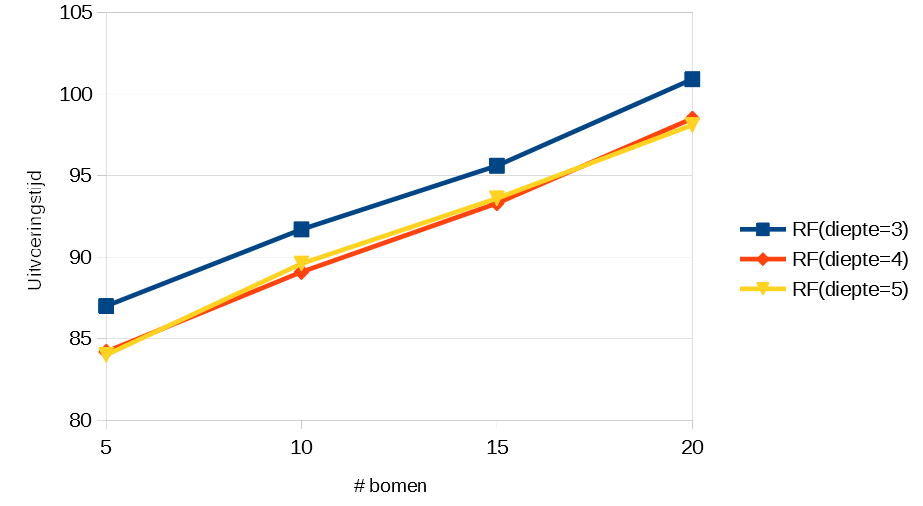
\includegraphics[width=\linewidth]{images/evaluatie/uitvoeringstijdrf.png}
\end{subfigure}
\caption{De invloed van diepte en aantal bomen op de uitvoeringstijd van DT en RF}
\label{fig:invloed diepte en aantal bomen uitvoeringstijd}
\end{figure}
\newpage
\section{Stochatisch bijleren}
In de onderstaande tabellen (tabellen \ref{tab:resultaten stochastisch bijleren PA}-\ref{tab:resultaten stochastisch bijleren RF}) zijn de resultaten te zien van gelijkaardige testen zoals in deel 2 van dit hoofdstuk. Het enige verschil met de voorgaande test, is de update-strategie voor het updaten van de verschillende modellen. Elke iteraties is er een kans $P(u_c|\Delta_c)$ gebaseerd op het verschil tussen de voorspelde cadans en de FCC.
\\\\
In het vorig hoofdstuk (sectie 2.3.1) werden verwachtingen opgesteld rond deze testen. Er werd verwacht dat de modellen deze probabilistische update-strategie aankunnen. In sommige gevallen is de MSE gelijkaardig aan de resultaten van de testen in deel 2 van dit hoofdstuk (PA-I, PA-II en RF en DT met diepte drie). Alle andere gevallen vertonen een betere MSE dan de originele testen. Dit komt waarschijnlijk door de hoeveelheid trainingsdata die gebruikt wordt. De probabilistische update-strategie zorgt ervoor dat er meer wordt bijgeleerd, waardoor er meer data beschikbaar is. De verwachting dat de modellen stochastisch kunnen bijleren is dus deels correct. Bomen van diepte drie moeten echter veel meer leren (aangezien $\Delta_c$ hoger is). Deze keer valt er wel een verschil te zien tussen een klein RF en een groot RF. Een groter RF traint minder vaak.
\\\\
Bij DT en RF is de stijging van het gemiddeld aantal keer trainen het grootst. PA presteerde al slechter dan de andere modellen waardoor de stijging hier minder extreem is. De algemene stijging is te wijten aan het feit dat er geen tolerantiegrens meer is. Het verschil tussen de voorspelde cadans en het fietsersmodel ($\Delta_c$) kan maar enkele rpm groot zijn, het kan nog steeds een update veroorzaken. Figuur \ref{fig:stochastic diff rf} toont hoe $\Delta_c$ evolueert doorheen de test voor een RF bestaande uit 20 bomen met diepte vier. Dit model update gemiddeld 59.6 keer. Aan de grafiek te zien zijn deze updates meestal doorgevoerd wanneer het verschil klein is ($\Delta_c<2$).
 

\begin{table}[hp!]
\centering
\begin{tabular}{|l|l|l|l|l|l|}
\hline
\multicolumn{2}{|l|}{\multirow{2}{*}{Passive Aggressive Algorithm}}                               & \multicolumn{4}{c|}{c}                                        \\ \cline{3-6} 
\multicolumn{2}{|l|}{}                                                                            & 1             & 2             & 5             & 10            \\ \hline
\multirow{2}{*}{Gemiddelde MSE}                                                           & PA-I  & 14.76 (+1\%)  & 14.63 (+5\%)  & 14.66 (+7\%)  & 14.60 (+10\%) \\ \cline{2-6} 
                                                                                          & PA-II & 14.52 (+7\%)  & 14.50 (+6\%)  & 14.05 (-1\%)  & 15.56 (+15\%) \\ \hline
\multirow{2}{*}{\begin{tabular}[c]{@{}l@{}}Gemiddeld aantal \\ keer trainen\end{tabular}} & PA-I  & 175.6 (+42\%) & 170.3 (+48\%) & 148.8 (+26\%) & 147.7 (+28\%) \\ \cline{2-6} 
                                                                                          & PA-II & 170.3 (+46\%) & 168.1 (+45\%) & 176.0 (+53\%) & 179.0 (+54\%) \\ \hline
\end{tabular}
\caption{Resultaten stochastisch bijleren PA}
\label{tab:resultaten stochastisch bijleren PA}
\end{table}

\begin{table}[hp!]
\begin{tabular}{|l|l|l|l|}
\hline
\multirow{2}{*}{Decision tree}                                           & \multicolumn{3}{c|}{Diepte}                    \\ \cline{2-4} 
                                                                         & 3              & 4             & 5             \\ \hline
Gemiddelde MSE                                                           & 9.37\phantom{1} (-8\%)    & 2.41 (-33\%)  & 1.06 (-37\%)  \\ \hline
\begin{tabular}[c]{@{}l@{}}Gemiddeld aantal \\ keer trainen\end{tabular} & 160.8 (+341\%) & 88.9 (+640\%) & 51.3 (+342\%) \\ \hline
\end{tabular}
\caption{Resultaten stochastisch bijleren beslissingsboom}
\label{tab:resultaten stochastisch bijleren DT}
\end{table}

\begin{table}[htp!]
\centering
\begin{tabular}{|l|l|l|l|l|l|}
\hline
\multicolumn{2}{|l|}{\multirow{2}{*}{Random forest}}                                                 & \multicolumn{4}{c|}{Aantal bomen}                                 \\ \cline{3-6} 
\multicolumn{2}{|l|}{}                                                                               & 5              & 10             & 15             & 20             \\ \hline
\multirow{3}{*}{Gemiddelde MSE}                                                           & Diepte 3 & 7.35 (+5\%)    & 7.42 (+2\%)    & 7.33 (+9\%)    & 7.37 (+12\%)   \\ \cline{2-6} 
                                                                                          & Diepte 4 & 1.47 (-48\%)   & 1.38 (-38\%)   & 1.37 (-38\%)   & 1.35 (-50\%)   \\ \cline{2-6} 
                                                                                          & Diepte 5 & 0.56 (-69\%)   & 0.59 (-64\%)   & 0.53 (-73\%)   & 0.56 (-63\%)   \\ \hline
\multirow{3}{*}{\begin{tabular}[c]{@{}l@{}}Gemiddeld \\ aantal keer \\ trainen\end{tabular}} & Diepte 3 & 145.3 (+578\%) & 143.8 (+615\%) & 145.4 (+707\%) & 144.7 (+704\%) \\ \cline{2-6} 
                                                                                          & Diepte 4 & 72.8\phantom{1} (+511\%)  & 58.2\phantom{1} (+380\%)  & 61.6\phantom{1} (+413\%)  & 59.6\phantom{1} (+409\%)  \\ \cline{2-6} 
                                                                                          & Diepte 5 & 40.4\phantom{1} (+236\%)  & 31.8\phantom{1} (+167\%)  & 33.4\phantom{1} (+185\%)  & 30.4\phantom{1} (+169\%)  \\ \hline
\end{tabular}
\caption{Resultaten stochastisch bijleren random forest}
\label{tab:resultaten stochastisch bijleren RF}
\end{table}




\begin{figure}[hp]
	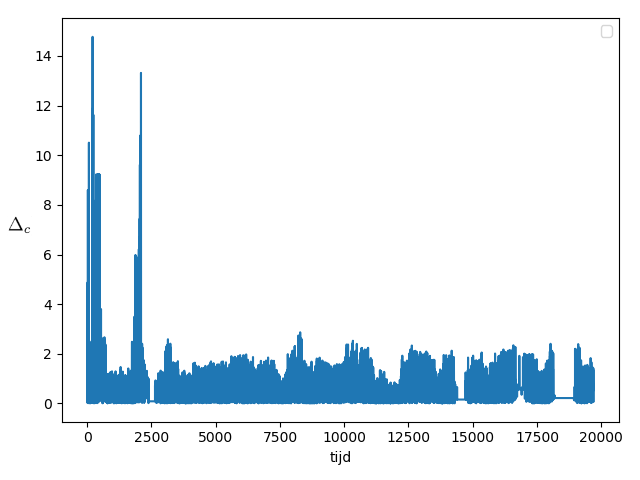
\includegraphics[width=\linewidth]{images/evaluatie/stochastic_diff_rf.png}
	\caption{Het absoluut verschil tussen het fietsersmodel en de voorspellingen ($\Delta_c$) in verloop van tijd}
	\label{fig:stochastic diff rf}
\end{figure}
\newpage
\section{Conceptuele drift}
Wederom wordt dezelfde test als in deel 2 van dit hoofdstuk gebruikt als basis om resultaten te verkrijgen van de twee algoritmes die omgaan met conceptuele drift. Het model voor deze test is een RF bestaande uit 20 bomen met diepte vier. Eerst wordt het RF getraind op basis van een fietsersmodel in functie van het DC-koppel (gemiddeld koppel) voor 20000 iteraties. Vervolgens “stopt” de fiets en wordt het fietsersmodel vervangen door één in functie van de helling. Deze nieuwe actor fietst dan voor 40000 iteraties. De tweede fietstocht is langer genomen om na te gaan of de datastructuren wel groot genoeg zijn zodat het hele concept in deze structuur past. Er worden vier verschillende groottes (500, 750, 1000 en 1250) met elkaar vergeleken die respectievelijk overeenkomen met data voor 10, 15, 20 en 25 trainingen. Deze worden dan vergeleken met een referentietest, een uitvoering zonder drift technieken. 
\\\\
In figuur \ref{fig:conceptuele drift vergelijking} is te zien dat wanneer er minder data wordt bijgehouden, er in totaal minder moet geleerd worden. Dit verschilt met de verwachting, die opgesteld is in sectie 2.4.4, dat kleinere structuren slechter zouden presteren dan grotere structuren. Waarschijnlijk is het betere resultaat juist te wijten aan de kleine structuur waardoor er snel vergeten wordt. In grotere structuren blijft data langer rondhangen. Het oude concept vult niet de hele structuur. Hierdoor zal er meerdere keren geüpdatet moet worden vooraleer het nieuwe concept geleerd is, net zoals wanneer er geen drift mechanisme is. Uiteindelijk is het oude concept vergeten, maar hiervoor was er veel meer data nodig. Bijvoorbeeld, bij het veranderen van concept hebben we twee of drie keer zoveel data nodig van situatie A, die ook voorkomt tijdens de vorige fietstocht (situatie is hier de algemene toestand van de fiets). Vervolgens komt situatie B die weeral twee of drie keer zoveel data nodig heeft omdat het statisch schuivend venster nog niet genoeg vergeten heeft. Uiteindelijk hebben we zoveel data toegevoegd van het nieuwe concept dat het oude concept helemaal vergeten is. Maar omdat er zoveel meer data nodig was, zijn nog niet alle situaties bekeken. Als de fiets dan in een ongeziene situatie komt, kan data van situatie A al vergeten worden. Stel dat situatie A uiteindelijk terugkomt, dan moet dit opnieuw geleerd worden. Deze keer minder aangezien er geen conflict is met een ouder concept. Dit probleem is zichtbaarder in een statisch schuivend venster dan bij sampling aangezien sampling ``sneller" data vergeet. Elke keer er een observatie toegevoegd wordt, is er een kans dat er één verwijderd wordt. Waardoor elke situatie in mindere mate aanwezig is, maar toch nog genoeg om een goede voorspelling te leveren. Merk op dat voor zowel statisch schuivend venster als sampling bij grootte 500, er minstens 1750 observaties bekeken zijn om met conceptuele drift om te gaan.

\begin{figure}[th]
	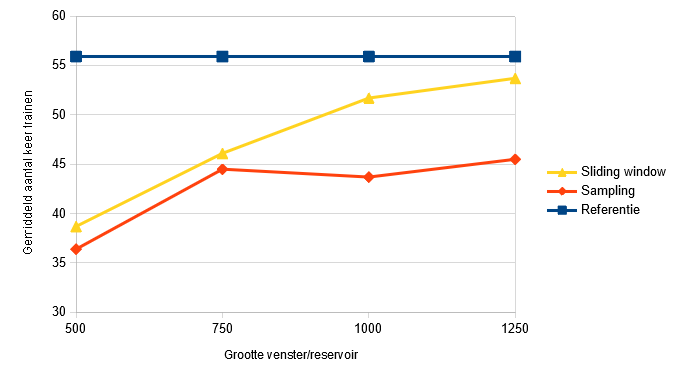
\includegraphics[width=\linewidth]{images/evaluatie/conceptuele_drift_vergelijking.png}
	\caption{Resultaten van beide technieken om met conceptuele drift om te gaan.}
	\label{fig:conceptuele drift vergelijking}
\end{figure}

